\documentclass{article}
\usepackage[margin=1in]{geometry}
\usepackage{multicol}
\usepackage{graphicx}
\usepackage{wrapfig}
\usepackage{lipsum}
\usepackage{amsmath}
\usepackage{hyperref}
\title{Measuring the Speed Of Sound In Air Using Sonar From Mobile Phones}
\author{\normalsize Lourenz Baliber \\ \normalsize Department of Physics, University of San Carlos, Cebu City 6000, Philippines \\ \normalsize 20102966@usc.edu.ph}

\begin{document}
\maketitle

\begin{abstract}
\noindent Under normal atmospheric pressure above sea level at $T=31^{\circ}C$, the time delay at specific distances between the transmitted and reflected sound wave was recorded with the help of a smartphone application. Using the data, the determination of the speed of sound in air was obtained. The result, $v_{s} = 337.64 \, m \, s^{-1}$, is in close proximity to the accepted value $349.6 \, m \, s^{-1}$.
\end{abstract}

\begin{multicols}{2}
\section{Introduction}
\paragraph{}

Most bats live in caves. Yet, despite not being able to see in pitch black darkness, bats are known to acrobatically navigate and hunt. In order to perform such feats, they make high-pitched sounds and listen for echoes using their ears. . This is also known echolocation \cite{bats}. Dolphins and other animals also use this technique in order to determine the location of objects. With sound, a lot of things can be done. It is used for communication, music, art, transportation, etc. Most importantly, it is used in physics experiments.

For example, three-dimensional (3D) imaging sonars are used in ocean exploration and exploitation and are becoming highly relevant \cite{sonar}. Sonars are commonly used in detection or navigation but it can also be used to calculate the speed of sound. By determining the distance of an object from a source and calculating the time delay, it is possible to measure the speed of sound in air. In this undertaking, the use of sonar using a mobile application in the determination of the speed of sound in air is presented.  
\section{Theoretical Background}
\paragraph{}

Theoretically, the speed of sound in relation to temperature is given by the equation:

\begin{equation}\label{eq:1}
v_{s}=331 \frac{m}{s}+(0.6 \frac{m}{s})/^{\circ}C * T
\end{equation} where $T$ is the ambient temperature. Sonar may also be used to estimate distances by using sound waves. Utilizing the relationship, 

\begin{equation}\label{eq:2}
d = v_{s}t
\end{equation} \indent The determination of the distance can be calculated. Since the distance traveled by the sound wave is the distance of transmitted and reflected sound wave, 

\begin{equation}\label{eq:3}
d = \frac{1}{2}d_{total}
\end{equation} taking half of the total distance from equation \eqref{eq:2} yields,

\begin{equation}\label{eq:4}
d = \frac{1}{2}v_{s}t_{delay}
\end{equation} \indent Solving for the the total distance traveled by the sound from the source is given by the equation:

\begin{equation}\label{eq:5}
2d = v_{s}t_{delay}
\end{equation} which shows a linear relationship between the total distance traveled by the sound from the source and the time delay and when plotted against each other $2d \, against \, t_{delay}$ gives $m$:

\begin{equation}\label{eq:6}
y = mx
\end{equation} where $y$ is $2d$, $x$ is $t_{delay}$ and $m$ is the slope of the linear plot and the experimental value of the speed of sound. 


\section{Experimental Procedure}
\paragraph{}
A tape measure, meter stick, foam, masking tape, flat trays and small white board composed the experimental setup which is shown in Figure 1. 

In performing the experiment, a smartphone-based sonar was launched through an app known as Phyphox \cite{phyphox}.

\begin{wrapfigure}{r}{4.5cm}
  \centering
    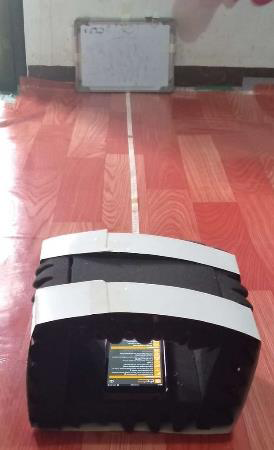
\includegraphics[scale=0.5]{setup.png}
  \caption{Experimental setup}
\end{wrapfigure}

As illustrated in Figure 1, a cavity was assembled using foams. Its size allowed enough room for the smartphone to be placed, while the cavity reduced unwanted disturbances from external noise. The constructed cavity was layed on the floor against a reflecting surface. Then, a tape measure was positioned on the floor to measure the distance between the smartphone and the reflecting surface. The cavity was set to a position where the microphone in the smartphone and the reflecting surface is $80 \, cm$ apart.

Using a smartphone, the Phyphox application was installed. After the installation, \textbf{Acoustics} $\rightarrow$ \textbf{Sonar} $\rightarrow$ \textbf{Timing} was chosen. With the help of the Phyphox GUI, the spikes in the echo strength graph was recorded in three significant figures. The procedures was then repeated for different distances: $90 \, cm, 100 \, cm, 110 \, cm, 120 \, cm$. 

\section{Data Analysis}
\paragraph{}

In the experiment, measuring the surrounding temperature gives $T = 31^{\circ}C$. Using equation \eqref{eq:1}, the locally accepted value of the speed of sound is $349.5 \, m \, s^{-1}$.

Five trials were made in the experiment. The independent variable, distance between the smartphone and the reflecting surface $2d$, and the dependent variable, time delay $t_{delay}$ were recorded in these five trials. 


\begin{center}
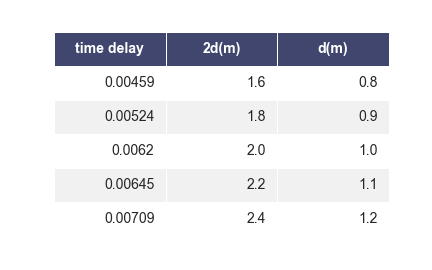
\includegraphics[scale=0.5]{table_mpl.png} 
Table 1: Measured time delay associated with the distance between the source and the reflecting surface.
\end{center}

The obtained dataset was recorded in Excel as shown in Table 1. By performing linear regression and setting the intercept into zero, the equation $y=337.64x$ was acquired as shown in Figure 2. Following equation \eqref{eq:6}, the experimental value of the speed of sound is  $337.64 \, m \cdot s^{-1}$ 

\begin{center}
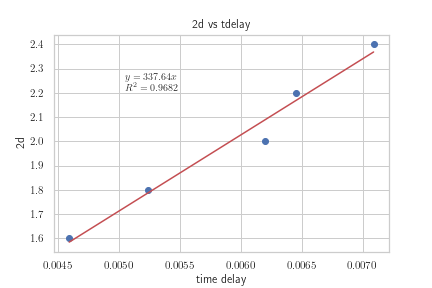
\includegraphics[scale=0.5]{output.png}
Figure 2: A scatterplot of the sum of the distance between the smartphone and the reflecting surface against time delay. The slope is $337.64 \, m \cdot s^{-1} $
\end{center}

For the calculation of error, regression data analysis in Excel was utilized as shown in Table 2. From the regression table in Excel, the equation of the slope without setting the intercept to zero is $y=313.69x+0.15$ which yields an error of $29.59$ while the error of the the slope when intercept is set to zero is $4.22$. 

\begin{center}
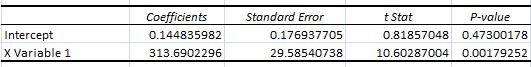
\includegraphics[scale=0.55]{error.JPG}\\
Table 2: Standard error from regression data analysis package in Excel.
\end{center}

Calculating for the percentage error of the value gives $3.42\%$ in comparison to the locally accepted value of $349.5 \, m \, s^{-1}$. However, for educational purposes, it is within tolerable limits.

\section{Conclusions and \\ Recommendations}
\paragraph{}

The obtained value for the speed of sound is satisfactory and is also consistent with the accepted value using equation \eqref{eq:1}. The errors in the activity was caused by unnecessary noises from external sources. Nonetheless, the experiment proved that sonar can be used in the determination of the speed of sound in air. Thus, as a suggestion, a quiet environment is required for a more accurate calculation.

\section*{Acknowledgement}
\paragraph{}

The completion of this project could not have been feasible without the assistance of Sir Unofre Pili and his exemplary teaching. The author also acknowledges his family and classmates for their guidance and support.


\begin{thebibliography}{9}

\bibitem{bats}
Carolyn Wilke. 2020 Here’s what bats ‘see’ when they explore the world with sound . \href{https://www.sciencenewsforstudents.org/article/what-bats-see-when-they-probe-the-world-with-sound}{https://www.sciencenewsforstudents.org/article/what-bats-see-when-they-probe-the-world-with-sound}

\bibitem{sonar}
Peng W. ,et al. 2021 . Improving performance of three-dimensional imaging sonars through deconvolution

\bibitem{phyphox}
\textit{Phyphox}. \href{https://phyphox.org/}{https://phyphox.org/}

\bibitem{pili} 
Pili U. 2020 Sound-based measurement of g using
a door alarm and a smartphone: listening to the simple
pendulum Phys. Educ. 55 033001

\bibitem{knuthwebsite} 
Knuth: Computers and Typesetting,
\texttt{http://www-cs-faculty.stanford.edu/}

\bibitem{mpl} 
Hunter, J. D. 2007 Matplotlib: A 2D graphics environment Computing in Science \& Engineering ; 10.1109/MCSE.2007.55

\end{thebibliography}

\noindent \textbf{Lourenz Baliber} is a 1st year BS Applied Physics student in the University of San Carlos.
\begin{wrapfigure}{l}{4cm}
  \centering
  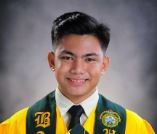
\includegraphics[scale=0.75]{grad pic.jpg} 
\end{wrapfigure}
This laboratory report, \textit{Measuring the Speed Of Sound In Air Using Sonar From Mobile Phones}, is a requirement for PHYS 1242.

\end{multicols}
\end{document}

















